
%Faced with the possibility of having to receive a significant number of Spaniards, the Minister of the Interior first requested a census of all public or private premises available in the departments, particularly those that could be used to house refugees (Note d'information du Ministère de l'Intérieur envoyée aux préfets le 26 janvier 1939). Secondly, he called for contact to be made with private initiatives—especially the Red Cross, but also other philanthropic organizations—with the aim of involving them in humanitarian efforts. Lastly, a cost estimate was requested for the construction of barracks in locations that met all necessary conditions for hygiene, sanitation, and supply \citep{perez_rodriguez_indeseables_2022}. 

According to the data, up to the month of July 1939, there were 990 camps in France, hospitals or shelter centres with Spanish exiles in France. Regarding the refugees, 167,932 were combatants, most of whom were spread over 10 concentration camps, 3 hospitals and 2 refugee centres. The rest, a little over 150,000 people, civilians of both sexes and of various ages, were spread over the numerous refugee centres that extended throughout French territory. Most of these centres were managed by the host country itself, while 73 were subsidised by other countries \citep{generalitat_de_catalunya_relacio_2020}. \Cref{fig:map_camps} displays the geographical distribution of internment camps across France in 1939. Camps were not concentrated in a single region but spread widely, with notable clusters in the southern departments near the Spanish border as well as in central and western France. The size of the circles reflects camp capacity, highlighting a particularly dense presence in the Pyrenean area where the first wave of refugees entered. This distribution suggests that exposure to refugees varied considerably across municipalities. 

\begin{figure}[h!]
  \centering
  \caption{Location of the refugee camps}
  \label{fig:map_camps}
  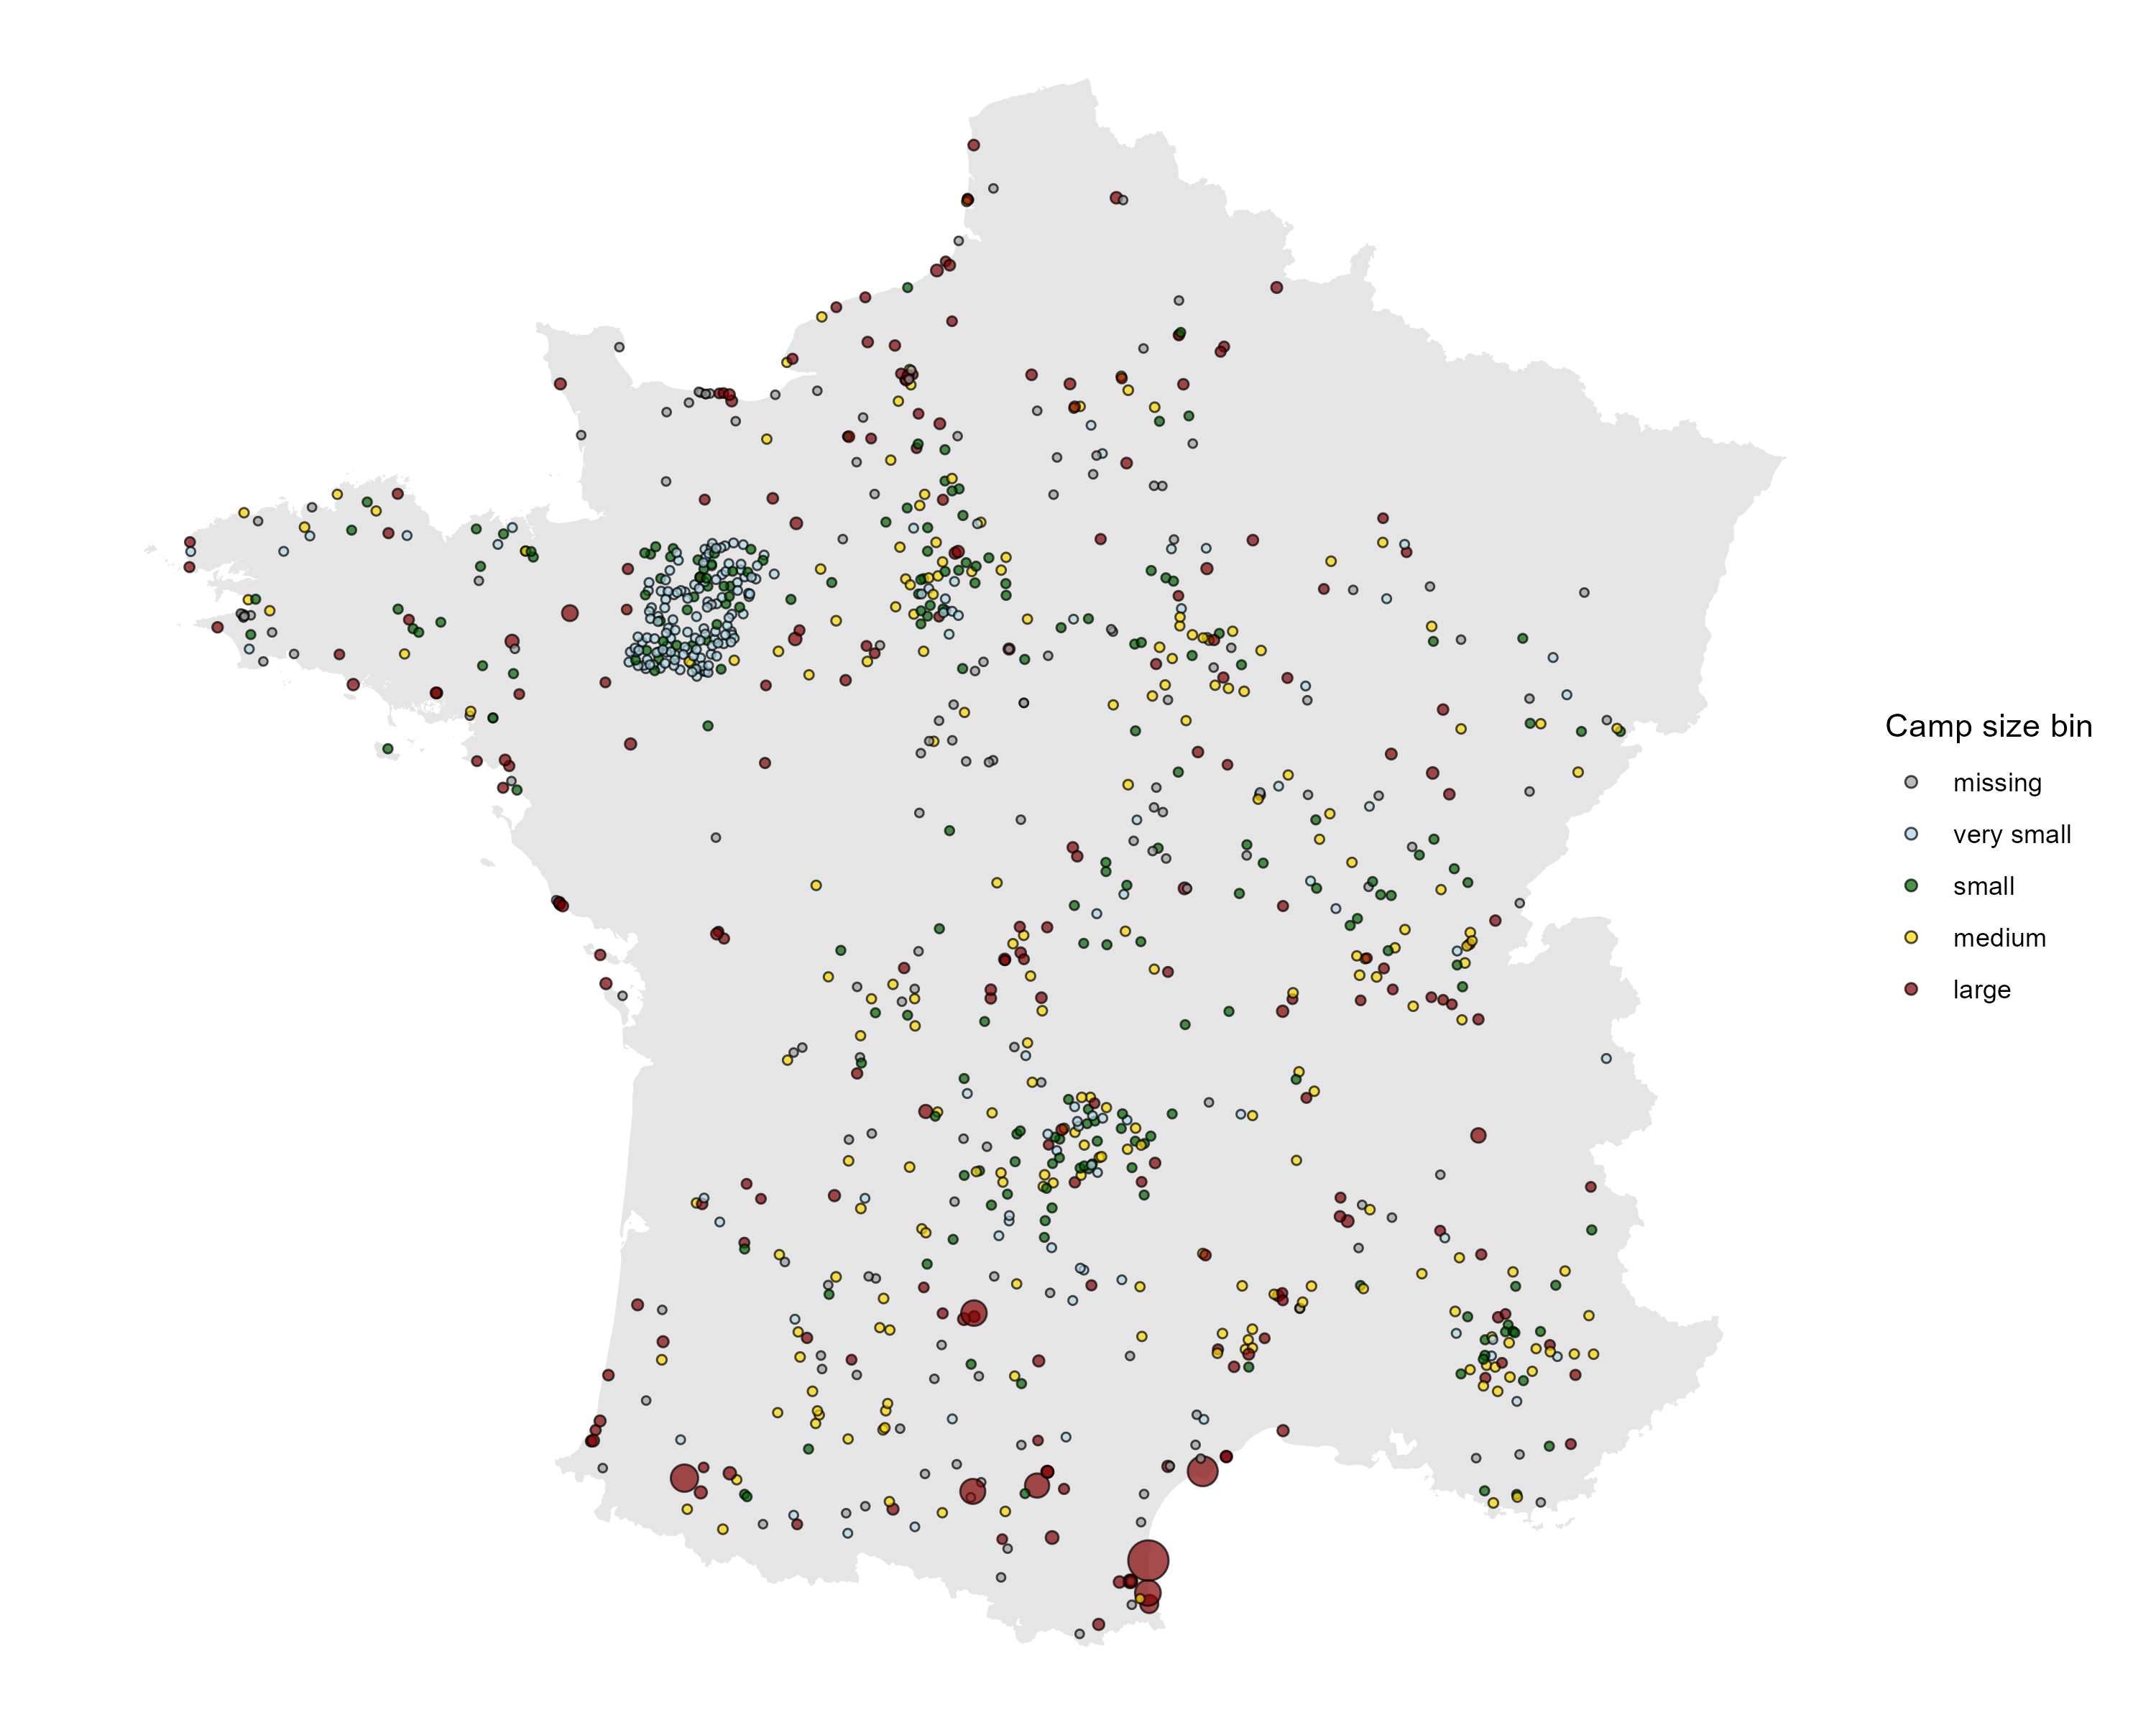
\includegraphics[width=0.8\linewidth]{figures/descriptives/maps/map7.png}
\end{figure}



\begin{figure}[h!]
    \caption{Locations of the Refugees Camps}
    \centering
    \begin{minipage}{0.49\textwidth}
        \centering
        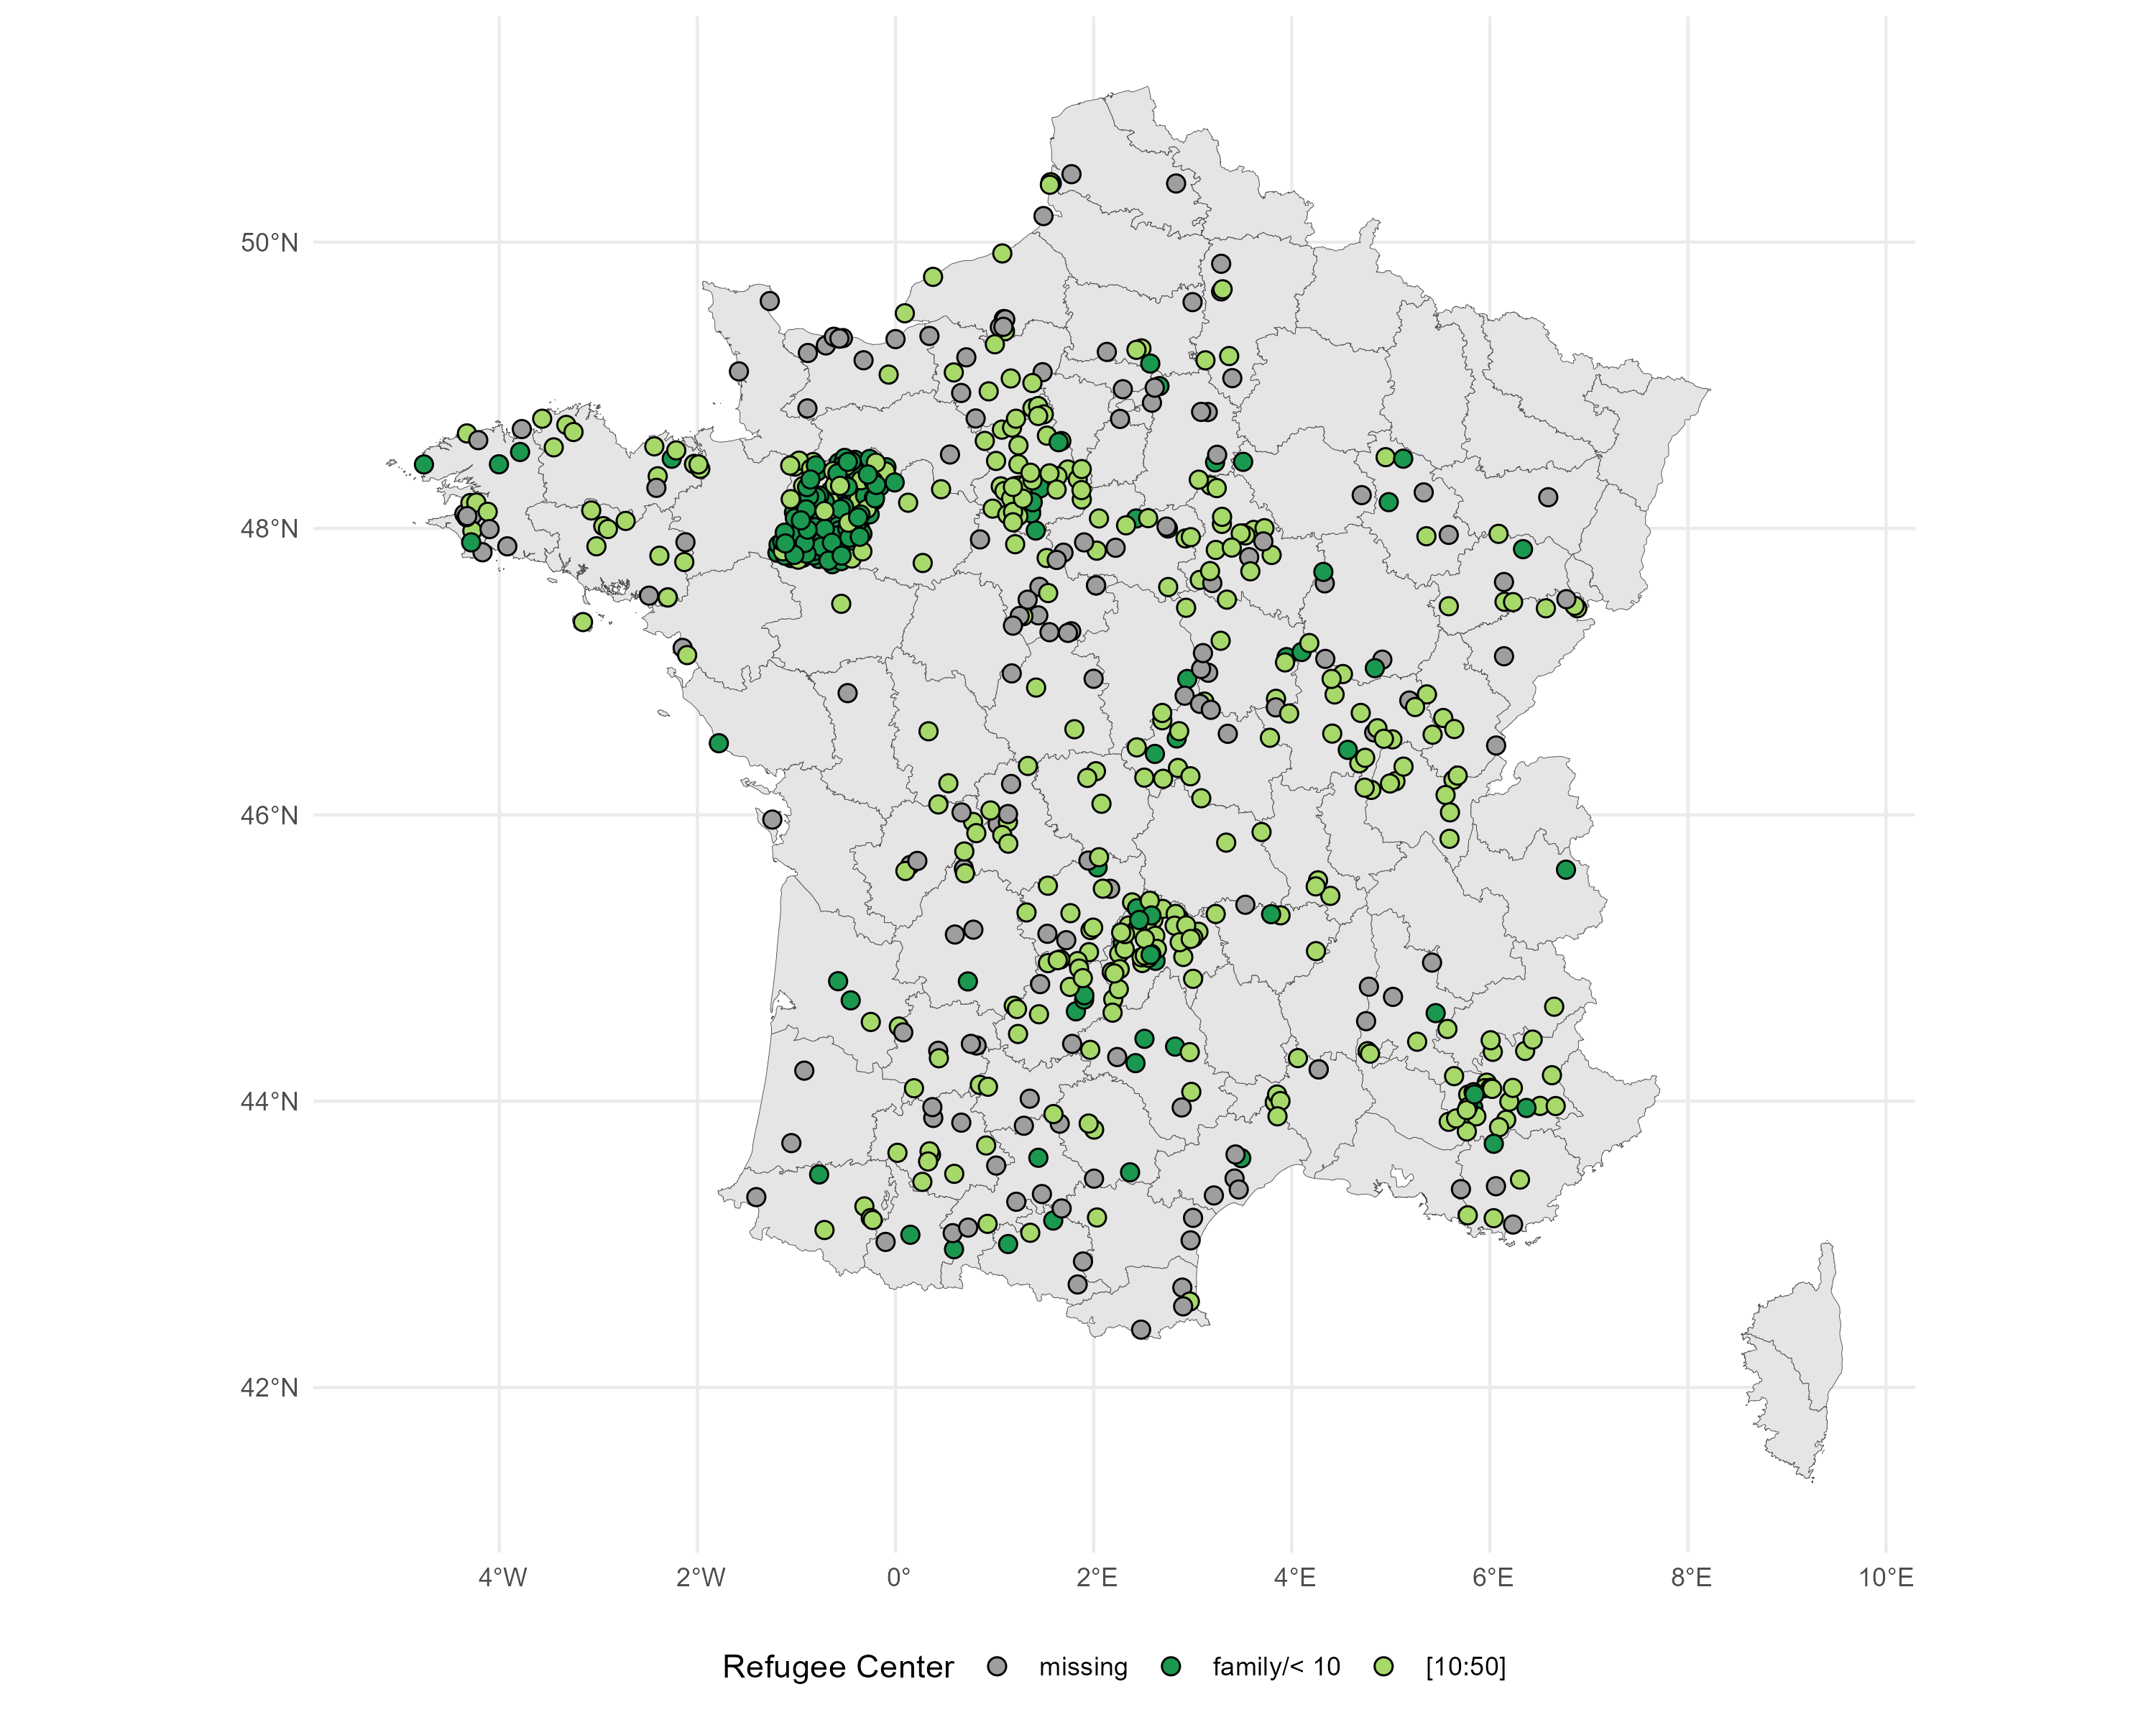
\includegraphics[width=\linewidth]{figures/descriptives/maps/map7.1.png}
        \subcaption{Missing, very small and small camps }
    \end{minipage}
    \hfill
    \begin{minipage}{0.49 \textwidth}
        \centering
        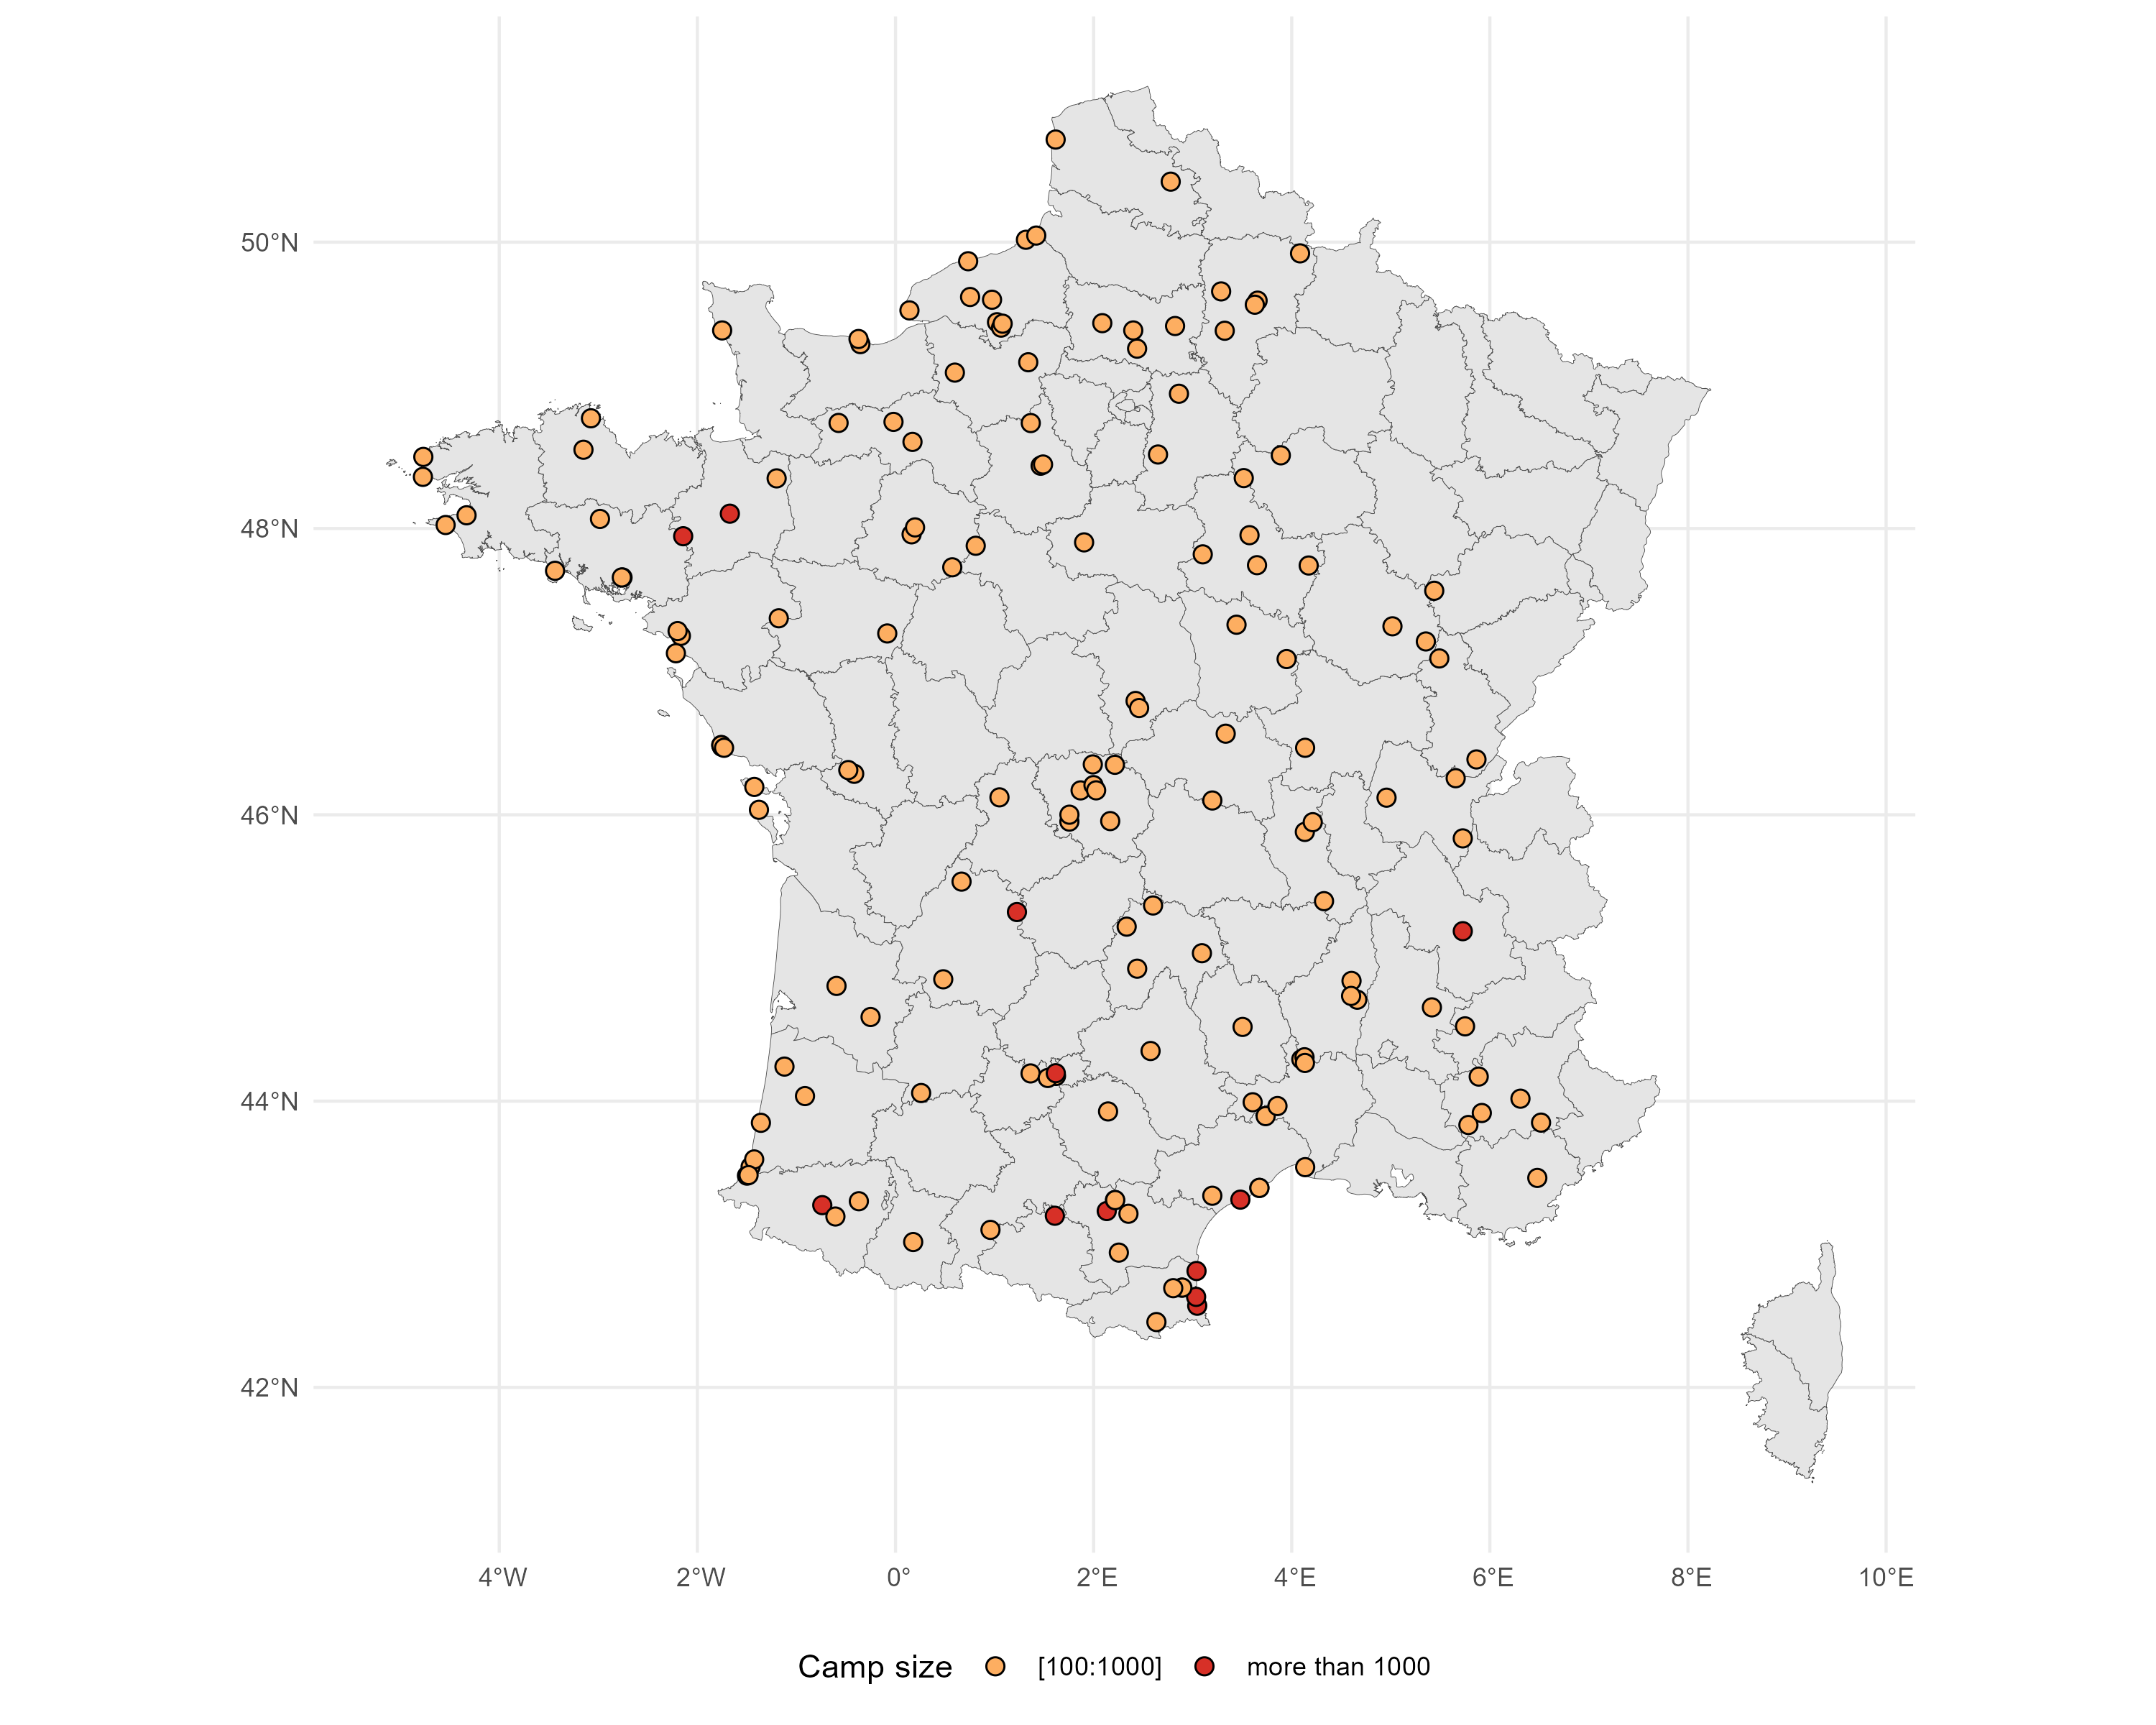
\includegraphics[width=\linewidth]{figures/descriptives/maps/map7.2.png}
        \subcaption{Medium and Large Size Camps}
    \end{minipage}
    \begin{minipage}{0.9\textwidth}
        \vspace{0.1in} 
        {\footnotesize Notes: The maps above display the locations of refugees camps across the French territory, per available information and size of camps. \par}
    \end{minipage}
\end{figure}




Table \ref{table:balance} reports balance statistics for the variables that are most relevant to assessing potential selection in the French dispersion policy. Because refugee placement was negotiated with departmental and municipal authorities, one concern is that more left-leaning municipalities may have been more willing to receive refugees; we therefore compare pre-war political orientation using the 1936 legislative results \citep{piketty_histoire_2023}. A second concern is municipality size: larger communes might have had more administrative capacity or available facilities, so we test for differences in population levels using historical census data \citep{insee_pop_hist_comm}. Another potential source of bias concerns the presence of other immigrant groups as the authorities may have avoided sending Spanish refugees to municipalities that had already received previous waves of foreigners. Because no city-level data on the share of the foreign population exist for this period, we approximate pre-existing immigrant presence using surname information from death records \citep{insee_deces_2025}. We identify French individuals with Spanish, Italian, or Portuguese surnames and recover their municipality of birth. From the same source, we also construct the share of women aged over twenty-one among the total population in the same age range. Balance in this measure is key considering women became eligible to vote in 1945. This does not pose a concern as long as treated and control municipalities exhibit comparable demographic structures.

Housing availability may have been another potential determinant of camp locations so we include a measure of buildings constructed by 1939 \citep{insee1968logements}. The Ministry of the Interior explicitly encouraged cooperation with private organisations such as the Red Cross and local philanthropic associations so we incorporate a measure of associative activity based on the legal registry of organisations \citep{dila_journalofficiel_portal}. Finally, we include variables capturing geographic and economic structure—altitude, precipitation, and mining activity \citep{pauling2006,camino2021}. Together, these variables allow us to test whether treated and control municipalities differed along the observable dimensions that could plausibly have influenced camp placement under the 1939 dispersion system.

Overall, observable characteristics are broadly similar across the two groups. Treated municipalities exhibit slightly higher support for the SFIO and the PCF, higher share of people with Italian-surnames, higher presence of mines and buildings per capita. Meanwhile, absolute standardized differences are below the conventional threshold of 0.25 \citep{ImbensRubin2015}. The exception is population, what we account for considering as an outcome share of votes with respect to total number of votes. 

\begin{table}[h!]
    \centering
    \caption{Balance test for municipalities with and without camps}
    \resizebox{0.8\textwidth}{!}{
    % latex table generated in R 4.5.0 by xtable 1.8-4 package
% Fri Mar  6 12:14:41 2026
\begin{tabular}{lrrrrr}
  \toprule
Variable & Mean Treated & SD Treated & Mean Control & SD Control & Abs. Norm. Diff \\ 
  \midrule
SFIO & 0.194 & 0.205 & 0.177 & 0.189 & 0.082 \\ 
  RAD SOC & 0.189 & 0.205 & 0.198 & 0.209 & 0.046 \\ 
  DIV & 0.001 & 0.008 & 0.006 & 0.053 & 0.108 \\ 
  FR URD & 0.133 & 0.235 & 0.159 & 0.252 & 0.108 \\ 
  DVG & 0.004 & 0.040 & 0.002 & 0.028 & 0.057 \\ 
  PCF & 0.104 & 0.126 & 0.085 & 0.114 & 0.161 \\ 
  DVD & 0.018 & 0.091 & 0.015 & 0.084 & 0.034 \\ 
  AGR & 0.009 & 0.052 & 0.019 & 0.080 & 0.148 \\ 
  USR & 0.071 & 0.151 & 0.069 & 0.154 & 0.013 \\ 
  AD & 0.277 & 0.245 & 0.270 & 0.271 & 0.028 \\ 
  Italian-origin surnames (share) & 0.167 & 0.042 & 0.165 & 0.064 & 0.022 \\ 
  Spanish-origin surname (share) & 0.064 & 0.038 & 0.064 & 0.048 & 0.000 \\ 
  Portuguese-origin surname (share) & 0.002 & 0.004 & 0.002 & 0.007 & 0.039 \\ 
  Associations (per capita) & 0.003 & 0.003 & 0.004 & 0.007 & 0.227 \\ 
  Presence of mines & 0.115 & 0.319 & 0.085 & 0.279 & 0.100 \\ 
  Buildings per capita & 0.319 & 0.113 & 0.308 & 0.097 & 0.109 \\ 
  Altitude & 262.237 & 279.532 & 279.950 & 296.883 & 0.061 \\ 
  Population & 3925.122 & 14860.324 & 941.338 & 3854.599 & 0.275 \\ 
  Mean rainfall & 807.804 & 160.548 & 817.462 & 163.060 & 0.060 \\ 
  WWI death rate & 3.776 & 1.370 & 4.093 & 3.440 & 0.121 \\ 
  Share of women 1936 & 0.575 & 0.043 & 0.571 & 0.062 & 0.060 \\ 
  Share of women 1945 & 0.555 & 0.035 & 0.553 & 0.052 & 0.047 \\ 
   \bottomrule
\end{tabular}
}
    \label{table:balance}
\begin{minipage}{0.8\textwidth}
        \vspace{0.5em}
\footnotesize
\textit{Notes:} All variables are measured before 1939, except for buildings per capita that includes 1939 due to limitations in the census. Electoral outcomes correspond to the 1936 legislative elections. 
\end{minipage}

\end{table}
